\chapter{Arhitektura i dizajn sustava}

{Arhitektura programske potpore predstavlja strukturu sustava ili više njih koji sadrži elemente, njihova obilježja i odnose među njima. Koristimo objektno orijentiranu arhitekturu koja najbolje odgovara razvoju složene web aplikacije namijenjene za više korisnika u stvarnom vremenu. Možemo ju klasificirati na četiri ključna dijela koji osiguravaju izvršavanje naredbi korisnika:

\begin{packed_item}
				\item \text{1. Web preglednik}
				\item \text{2. Web poslužitelj}
				\item \text{3. Web aplikacija}
				\item \text{4. Baza podataka}
			\end{packed_item}

% TODO: \usepackage{graphicx} required
				\begin{figure}[H]
					\centering
					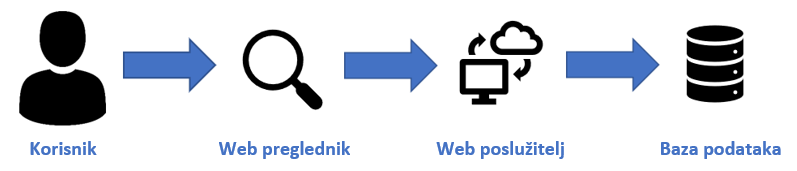
\includegraphics[width=1\linewidth]{"slike/arhitekturaApp.png"}
					\caption{Arhitektura sustava}
					\label{fig:arhitektura-sustava}
				\end{figure}

Prilikom pristupa web aplikaciji korisniku na jednostavan način postaje moguće pretražiti putovanja s odabranog polazišnog stajališta i kupiti kartu. Da bi korisnik mogao pristupiti navedenim funkcionalnostima treba pristupiti web pregledniku koji za njega vrši daljnju interakciju s ostalim podsustavima koji su sastavni dijelovi arhitekture sustava. Web preglednik dalje mora komunicirati s web poslužiteljem na kojem je sama implementacija web aplikacije. Preko web poslužitelja se obavljaju svi mogući funkcionalni zahtjevi aplikacije koji su prethodno definirani, a oni su izravno povezani s poslužiteljem baze podataka. U bazi podataka pohranjeni su svi podaci nužni za potpuno ispravan rad aplikacije, ali i podaci koje ručno unose korisnici poput osobnih podataka. Web poslužitelj šalje objekte na zahtjev klijenata, ti se zahtjevi realiziraju u obliku HTTP poruka. Web poslužitelju se pristupa preko nekog web preglednika.

Za izradu frontend dijela web aplikacije korišten je programski jezik Javascript s razvojnim okvirom React.js. Za izradu backend dijela korišten je Typescript s razvojnim okvirom Express.js. Baza podataka je implementirana pomoću PostrgreSQL.

 Za realizaciju arhitekture sustava korišten je koncept Model-View-Controller. Model–View–Controller je obrazac koji razdvaja aplikaciju u tri glavne
logičke komponente: Model, View i Controller. Svaka od nabrojenih komponenti ima zadatak rukovati s određenim razvojnim aspektima aplikacije. Također, one
su nezavisne jedna od druge i kao rezultat toga je jednostavno dodavanje i preoblikovanje svojstava.

\begin{figure}[H]
					\centering
					\includegraphics[width=0.7\linewidth]{"slike/MVC"}
					\caption{Model-View-Controller}
					\label{fig:Model-View-Controller}
				\end{figure}

• \textbf{Model}
Poznat je kao najniža razina što znači da je odgovoran za održavanje podataka s kojima korisnik radi. Glavni zadatak je dohvat, manipulacija podatcima odnosno suradnja s bazom podataka. 
Sprema tražene podatke u objekte i na taj način ih šalje bazi podataka. Reagira na zahtjeve Controllera jer on nikada sam ne razgovara s bazom podataka i nakon komunikacije
prosljeđuje potrebne podatke Controller-u. Jedna od bitnijih stvari za napomenuti je da Model nikada izravno ne komunicira s View.

• \textbf{View}
Služi za prikazivanje podataka tako što generira korisničko sučelje za korisnika. Ti podaci su rezultat rada Model-a, ali se oni ne preuzimaju izravno nego putem Controller-a tako da View surađuje samo s Controller-om.

•\textbf{Controller} 
Upravlja komponentama Model i View. Ne mora
brinuti o rukovanju logikom podataka, već samo govori Model-u što treba učiniti. Nakon primanja podataka od Model-a, on ih obrađuje i prosljeđuje rezultat do View-a.}

		
		\section{Baza podataka}
			
			
		{Za potrebe našeg sustava odabrali smo relacijsku bazu podataka koja nam olakšava modeliranje stvarnog svijeta. Baza je definirana skupom tablica, odnosno relacija koje su definirane svojim imenima i skupovima atributa (i ključevima). Zbog pouzdanosti, jednostavnosti i zadovoljavajućih preformansi, odabrali smo rad s PostreSQL bazom. Baza podataka omogućava nam brz i lak dohvat i spremanje podataka, odnosno obradu i izmjenu podataka korištenih u aplikaciji. Naša baza sastoji se od sljedećih entiteta: }
			\begin{packed_item}
				\item \text{User}
				\item \text{Ticket}
				\item \text{Journey}
				\item \text{TrainRoute}
				\item \text{Station}
				\item \text{SensorData}
			\end{packed_item}
		
			\subsection{Opis tablica}
			

\textbf{User}{ - Entitet User sadrži sve potrebne informacije o korisniku aplikacije koji može biti kupac ili administrator što određuje atribut UserType. User ima također i atribute firstName, lastName, email, password te createdDate što označava datum registracije korisnika. Email je jedinstven atribut, tako da se svaki User razlikuje po svom e-mailu. Ključ entiteta je email. }
				
				
				\begin{longtblr}[
					label=none,
					entry=none
					]{
						width = \textwidth,
						colspec={|X[6,l]|X[6, l]|X[20, l]|}, 
						rowhead = 1,
					} %definicija širine tablice, širine stupaca, poravnanje i broja redaka naslova tablice
					\hline \multicolumn{3}{|c|}{\textbf{Korisnik}}	 \\ \hline[3pt]
					\SetCell{LightGreen}email & VARCHAR	& jedinstveni e-mail korisnika   	\\ \hline
					firstName	& VARCHAR & ime korisnika \\ \hline 
					lastName & VARCHAR &  prezime korisnika \\ \hline 
					password & VARCHAR	&  lozinka registriranog korisnika	\\ \hline 
					role&VARCHAR&vrsta korisnika,može biti kupac ili administrator\\ \hline 
					createdDate&DATE&datum registracije korisnika 	\\ \hline 
				\end{longtblr}





\textbf{Ticket}{ - Entitet Ticket je slabi entitet koji ovisi o entitetu User iz razloga što karta ne može biti izdana bez da korisnik zatraži njezino izdavanje. Ključ entiteta Ticket je Id ticket-a. Atribut passengerEmail je strani ključ koji referencira entitet User te se radi o \textit{Many-to-Many} vezi. Atribut idJourney rute je strani ključ koji referencira entitet Journey te se radi o \textit{Many-To-One} vezi. }

				\begin{longtblr}[
					label=none,
					entry=none
					]{
						width = \textwidth,
						colspec={|X[6,l]|X[6, l]|X[20, l]|}, 
						rowhead = 1,
					} %definicija širine tablice, širine stupaca, poravnanje i broja redaka naslova tablice
					\hline \multicolumn{3}{|c|}{\textbf{Ticket}}	 \\ \hline[3pt]
					\SetCell{LightGreen}Id & INT	&  	jedinstveni identifikacijski broj karte koja je kupljena  	\\ \hline
					\SetCell{LightBlue} userId	& INT & strani ključ entiteta User 	\\ \hline 
					\SetCell{LightBlue} idJourney	& INT & strani ključ entiteta Journey \\ \hline
					passenger-Name	& VARCHAR & ime kupca karte \\ \hline 
					passenger-Surname & VARCHAR &  prezime kupca karte \\ \hline 
					wagon & INT	&  vagon za koji je kupljena karta \\ \hline
					wagonPosition & INT	&  pozicija vagona na kolodvoru	\\ \hline
					travelDate&DATE&datum putovanja 	\\ \hline
				\end{longtblr}
				
				


				\textbf{Journey} {- Ovaj entitet sadržava sve važne podatke za jedno putovanje vlakom. Sadrži atribute: IdJourney, departureTime i arrivalTime, price, departureStationName, arrivalStationName, routeId i sensorDataId. Atributi departureStationName i arrivalStationName su strani ključevi koji referenciraju entitet Station te se radi o \textit{Many-To-One} vezi. Atributi IdTrainRoute i sensorDataId su strani ključevi koji refenciraju entitet TrainRoute i SensorData putem \textit{Many-To-One} veze. }
				
				
				\begin{longtblr}[
					label=none,
					entry=none
					]{
						width = \textwidth,
						colspec={|X[6,l]|X[6, l]|X[20, l]|}, 
						rowhead = 1,
					} %definicija širine tablice, širine stupaca, poravnanje i broja redaka naslova tablice
					\hline \multicolumn{3}{|c|}{\textbf{Journey}}	 \\ \hline[3pt]
					\SetCell{LightGreen}idJourney & INT	&  	jedinstveni identifikacijski broj putovanja  	\\ \hline
					departureTime	& DATETIME &	datum i vrijeme polaska s polazišnog stajališta	\\ \hline 
					arrivalTime & DATETIME &	datum i vrijeme dolaska na odredišno stajalište	\\ \hline 
					price & FLOAT	&  	cijena karte za putovanje	\\ \hline 
					\SetCell{LightBlue} departure-StationName	&          VARCHAR &   	početno stajalište putovanja i strani ključ entiteta Station	\\ \hline 
					\SetCell{LightBlue} arrival-StationName	&        VARCHAR &   	završno stajalište putovanja	 i strani ključ entiteta Station	\\ \hline 
					\SetCell{LightBlue} idTrainRoute	& INT &   	jedinstveni identifikacijski broj TrainRoute-e	\\ \hline 
					sensorDataId	& INT &   	jedinstveni identifikacijski broj sensorData	\\ \hline
				\end{longtblr}
				
				





\textbf{TrainRoute} {- Entitet TrainRoute ima atribute: idTrainRoute, departureTime, arrivalTime, trainId i dates. U ruti Zagreb-Karlovac-Knin-Split, početak cjelokupne rute je Zagreb, a završetak Split. Entitet TrainRoute će imati sve moguće kombinacije podruta za primjer navedene rute. Journeys navedene rute će biti Zagreb-Karlovac, Zagreb-Knin, Zagreb-Split, Karlovac-Knin, Karlovac-Split, Knin-Split. Zbog potrebe zadatka da za svako putovanje imamo početno i završno odredište cjelokupne rute tog putovanja, nastao je ovaj entitet TrainRoute koji je povezan s Journeys \textit{One-To-Many} vezom. }
				
				
				\begin{longtblr}[
					label=none,
					entry=none
					]{
						width = \textwidth,
						colspec={|X[6,l]|X[6, l]|X[20, l]|}, 
						rowhead = 1,
					} %definicija širine tablice, širine stupaca, poravnanje i broja redaka naslova tablice
					\hline \multicolumn{3}{|c|}{\textbf{TrainRoute}}	 \\ \hline[3pt]
					\SetCell{LightGreen}IdTrainRoute & INT	&  	jedinstveni identifikacijski broj cjelokupne rute  	\\ \hline
					departureTime	& DATETIME &	datum i vrijeme polaska s polazišnog stajališta	\\ \hline 
					arrivalTime & DATETIME &	datum i vrijeme dolaska na odredišno stajalište	\\ \hline 
					trainId & INT	& jedinstveni identifikacijski broj vlaka koji vozi tu rutu 	\\ \hline 
					dates & DATETIME & datum vožnji vlaka \\ \hline
					
				\end{longtblr}

				\textbf{Station} {- Ovaj entitet sadržava imena svih stajališta. Entitet Stajalište povezan je putem dvije \textit{One-To-Many} veze s entitetom Putovanje, gdje jedna veza označava početno stajalište, a druga završno. }
				
				
				\begin{longtblr}[
					label=none,
					entry=none
					]{
						width = \textwidth,
						colspec={|X[6,l]|X[6, l]|X[20, l]|}, 
						rowhead = 1,
					} %definicija širine tablice, širine stupaca, poravnanje i broja redaka naslova tablice
					\hline \multicolumn{3}{|c|}{\textbf{Station}}	 \\ \hline[3pt]
					\SetCell{LightGreen}name & VARCHAR	&  	ime stajališta 	\\ \hline
				\end{longtblr}

				\textbf{SensorData} {- Ovaj entitet sadržava sve važne podatke za jedno mjerenje senzora. Sadrži atribute: id, time, speed, measurments, stationName, idJourney, idTrainRoute i travelDate. Entitet SensorData povezan je putem \textit{Many-To-One} veze s entitetom Journey. }
				
				
				\begin{longtblr}[
					label=none,
					entry=none
					]{
						width = \textwidth,
						colspec={|X[6,l]|X[6, l]|X[20, l]|}, 
						rowhead = 1,
					} %definicija širine tablice, širine stupaca, poravnanje i broja redaka naslova tablice
					\hline \multicolumn{3}{|c|}{\textbf{SensorData}}	 \\ \hline[3pt]
					\SetCell{LightGreen}id & INT	&  	jedinstveni identifikacijski broj mjerenja  	\\ \hline
					time & DATETIME & datum i vrijeme mjerenja senzora	\\ \hline 
					measurments & VARCHAR &	vrijednost mjerenja senzora	\\ \hline 			
					speed & INT &  	brzina vlaka u trenutku mjerenja senzora	\\ \hline 
					stationName	& VARCHAR &   	stanica koju je vlak prošao uz senzor	\\ \hline
					travelDate & DATE & datum putovanja vlaka koji prolazi kraj senzora  \\ \hline 
					\SetCell{LightBlue} idJourney	& INT &   	strani ključ entiteta Journey	\\ \hline 
					\SetCell{LightBlue} idTrainRoute	& INT &   	strani ključ entiteta TrainRoute	\\ \hline 
				\end{longtblr}
				
				

			\subsection{Dijagram baze podataka}

	
				% TODO: \usepackage{graphicx} required
				\begin{figure}[H]
					\centering
					\includegraphics[width=1\linewidth]{"slike/dijagramBaze"}
					\caption{Dijagram baze podataka}
					\label{fig:dijagram-bp}
				\end{figure}
			
			\eject
			
			
		\section{Dijagram razreda}
		
	

				% TODO: \usepackage{graphicx} required
				\begin{figure}[H]
					\centering
					\includegraphics[width=1\linewidth]{"slike/ModelClassDiagram"}
					\caption{Dijagram razreda Modela}
					\label{fig:dijagram-model}
				\end{figure}

				{Model razredi preslikavaju strukturu baze podataka u aplikaciji. Implementirane metode direktno komuniciraju s bazom podataka te vraćaju tražene podatke. Razred \textit{User} predstavlja registriranog i prijavljenog korisnika koji može koristiti njegove osnovne funkcionalnosti. Razred \textit{Ticket} predstavlja jednu kartu koju je kupio \textit{User} za jedno putovanje - \textit{Journey}. Razred \textit{Journey} predstavlja relaciju putovanja za koju korisnik(\textit{User}) kupuje željezničku kartu. Razred \textit{TrainRoute} predstavlja kompletnu rutu na kojoj putuje vlak na kojem je korisnik kupio kartu za određeno putovanje. Razred \textit{Station} predstavlja listu svih stajališta kojima vozi naš prijevoznik, a razred \textit{SensorData} predstavlja mjerenja sustava senzora Gotcha za svako putovanje.}

				% TODO: \usepackage{graphicx} required
				\begin{figure}[H]
					\centering
					\includegraphics[width=1\linewidth]{"slike/ControllerClassDiagram"}
					\caption{Dijagram razreda Controllera}
					\label{fig:dijagram-controller}
				\end{figure}
				{Dijagram se sastoji od 8 nadglednika: HomeController, LoginController, RegisterController, AdminController, PaymentController, SensorController, SettingsController, TimetableController te svi naslijeđuju apstraktni razred Controller. U serveru se inicijaliziraju svi kontroleri (stavljaju u listu). HomeController se koristi prilikom ulaska korisnika na Home ekran i prikaz voznog reda na stranici. RegisterController se koristi prilikom registracije korisnika na stranicu, a LoginController prilikom prijave korisnika/admina u stranicu. AdminController se koristi prilikom funkcionalnosti koje su omogućene za Admina(pregleda, brisanje korisnika).	SensorController se koristi prilikom dohvata i obrade podataka sa senzora. PaymentController služi za obradu plaćanja prilikom kupnje karta te sprema podatke o transakcijama. SettingsController koristimo pri dohvatu podataka korisnika te brisanju njegova računa. TimetableController koristimo pri dohvatu putovanja za odabranu odlaznu i dolaznu stanicu i datum.	}
			
			\eject

\section{Dijagram stanja}
			{Dijagram stanja opisuje dinamičko ponašanje dijela sustava u vremenu. Ono sadrži konačan broj stanja i prijelaza među stanjima temeljenima na događajima. Na slici je prikazan dijagram stanja za sve uloge korisnika: konkretnog korisnika i administratora. Početno stanje neregistriranog korisnika (odnosno neprijavljenog) vodi u stanje prijave. Neregistriranim korisnicima je ostavljena mogućnost registracije, nakon čega je prijavom moguće doći do početne stranice aplikacije. Uloga korisnika razdjeljuje stanje početne stranice na dva unutarnja. Administratorima je omogućena akcija prikaza svih korisnika, njihovog brisanja i ispisa njihovih transakcija. Konkretnim korisnicima je omogućena akcija ispisa nadolazećih vlakova na odabranu stanicu. Svi korisnici imaju i opciju prikaza voznog reda. Međutim, samo konkretni korisnici imaju opciju kupnje karte za odabrano putovanje. Da bi se izvršila kupnja potrebno je ispuniti obrazac (ukoliko nije upamćen jer se radi o prvoj transakciji) te ju potvrditi. Potvrdom se šalju dva e-maila, prvi za potvrdu o kupnji te drugi sa sadržajem karte i informacijama o odabranom putovanju. Iz svih stanja je moguće odjaviti se ili se vratiti u stanje početne stranice. } 
			
			 % TODO: \usepackage{graphicx} required
				\begin{figure}[H]
					\centering
					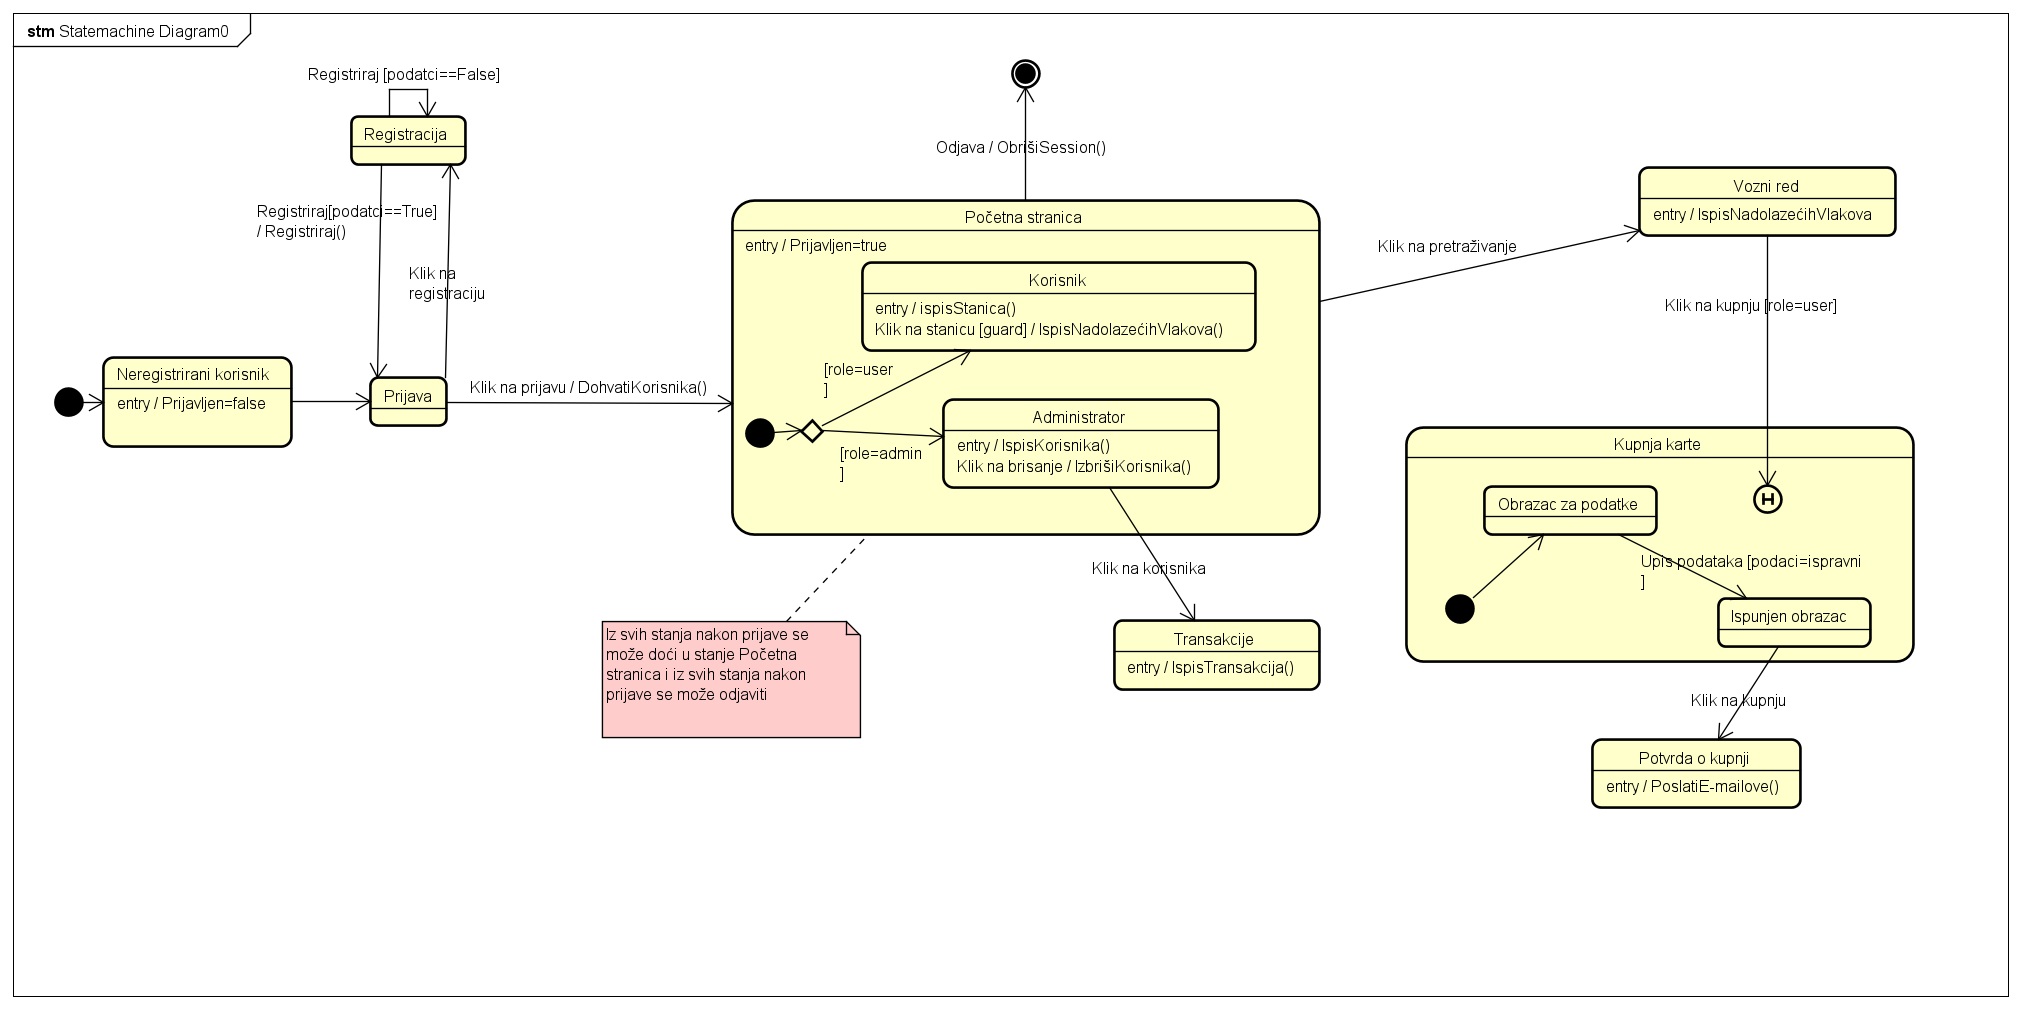
\includegraphics[width=1\linewidth]{"slike/StateMachineDiagram.png"}
					\caption{Dijagram stanja aplikacije}
					\label{fig:dij-state}
				\end{figure}
			
			
			\eject 
		
\section{Dijagram aktivnosti}

			{Dijagrami aktivnosti služe za modeliranje ponašanja nizom akcija, odnosno modeliranje toka i podataka. Pomaže nam pri zamišljanju redoslijeda aktivnosti i tijeka rada aplikacije. Na slici 4.7 prikazan je dijagram aktivnosti koji prikazuje procese pregledavanje i pretraživanje vlakova i voznih linija, odnosno kupnju karata za te linije. Korisnik se prijavljuje u sustav, zatim može pregledati vozni red pomoću odabira stanica i datuma polaska, te može pregledati koji vlakovi dolaze na označeno stajalište. Nakon odabira stanica i datuma dolazi do izlistanog voznog reda za te podatke pa odabire opciju kupnje. Zatim ispunjava obrazac za kartično plaćanje te potvrđuje svoju kupnju. Na slici 4.8 prikazan je dijagram aktivnosti administratora za brisanje korisnika i pregled njihovih transakcija. Nakon prijave, administrator dobiva izlistane korisnike za koje može odabrati brisanje ili pregled transakcija. Ukoliko odabere mogućnost brisanja, sustav će ga upozoriti i pitati je li siguran u brisanje toga klijenta. Administrator može prihvatiti brisanje ili odustati. Ako odabere pregled transakcija, aplikacija ga odvede na novu stranicu gdje su izlistane sve kupnje tog korisnika. }
			
			 % TODO: \usepackage{graphicx} required
				\begin{figure}[H]
					\centering
					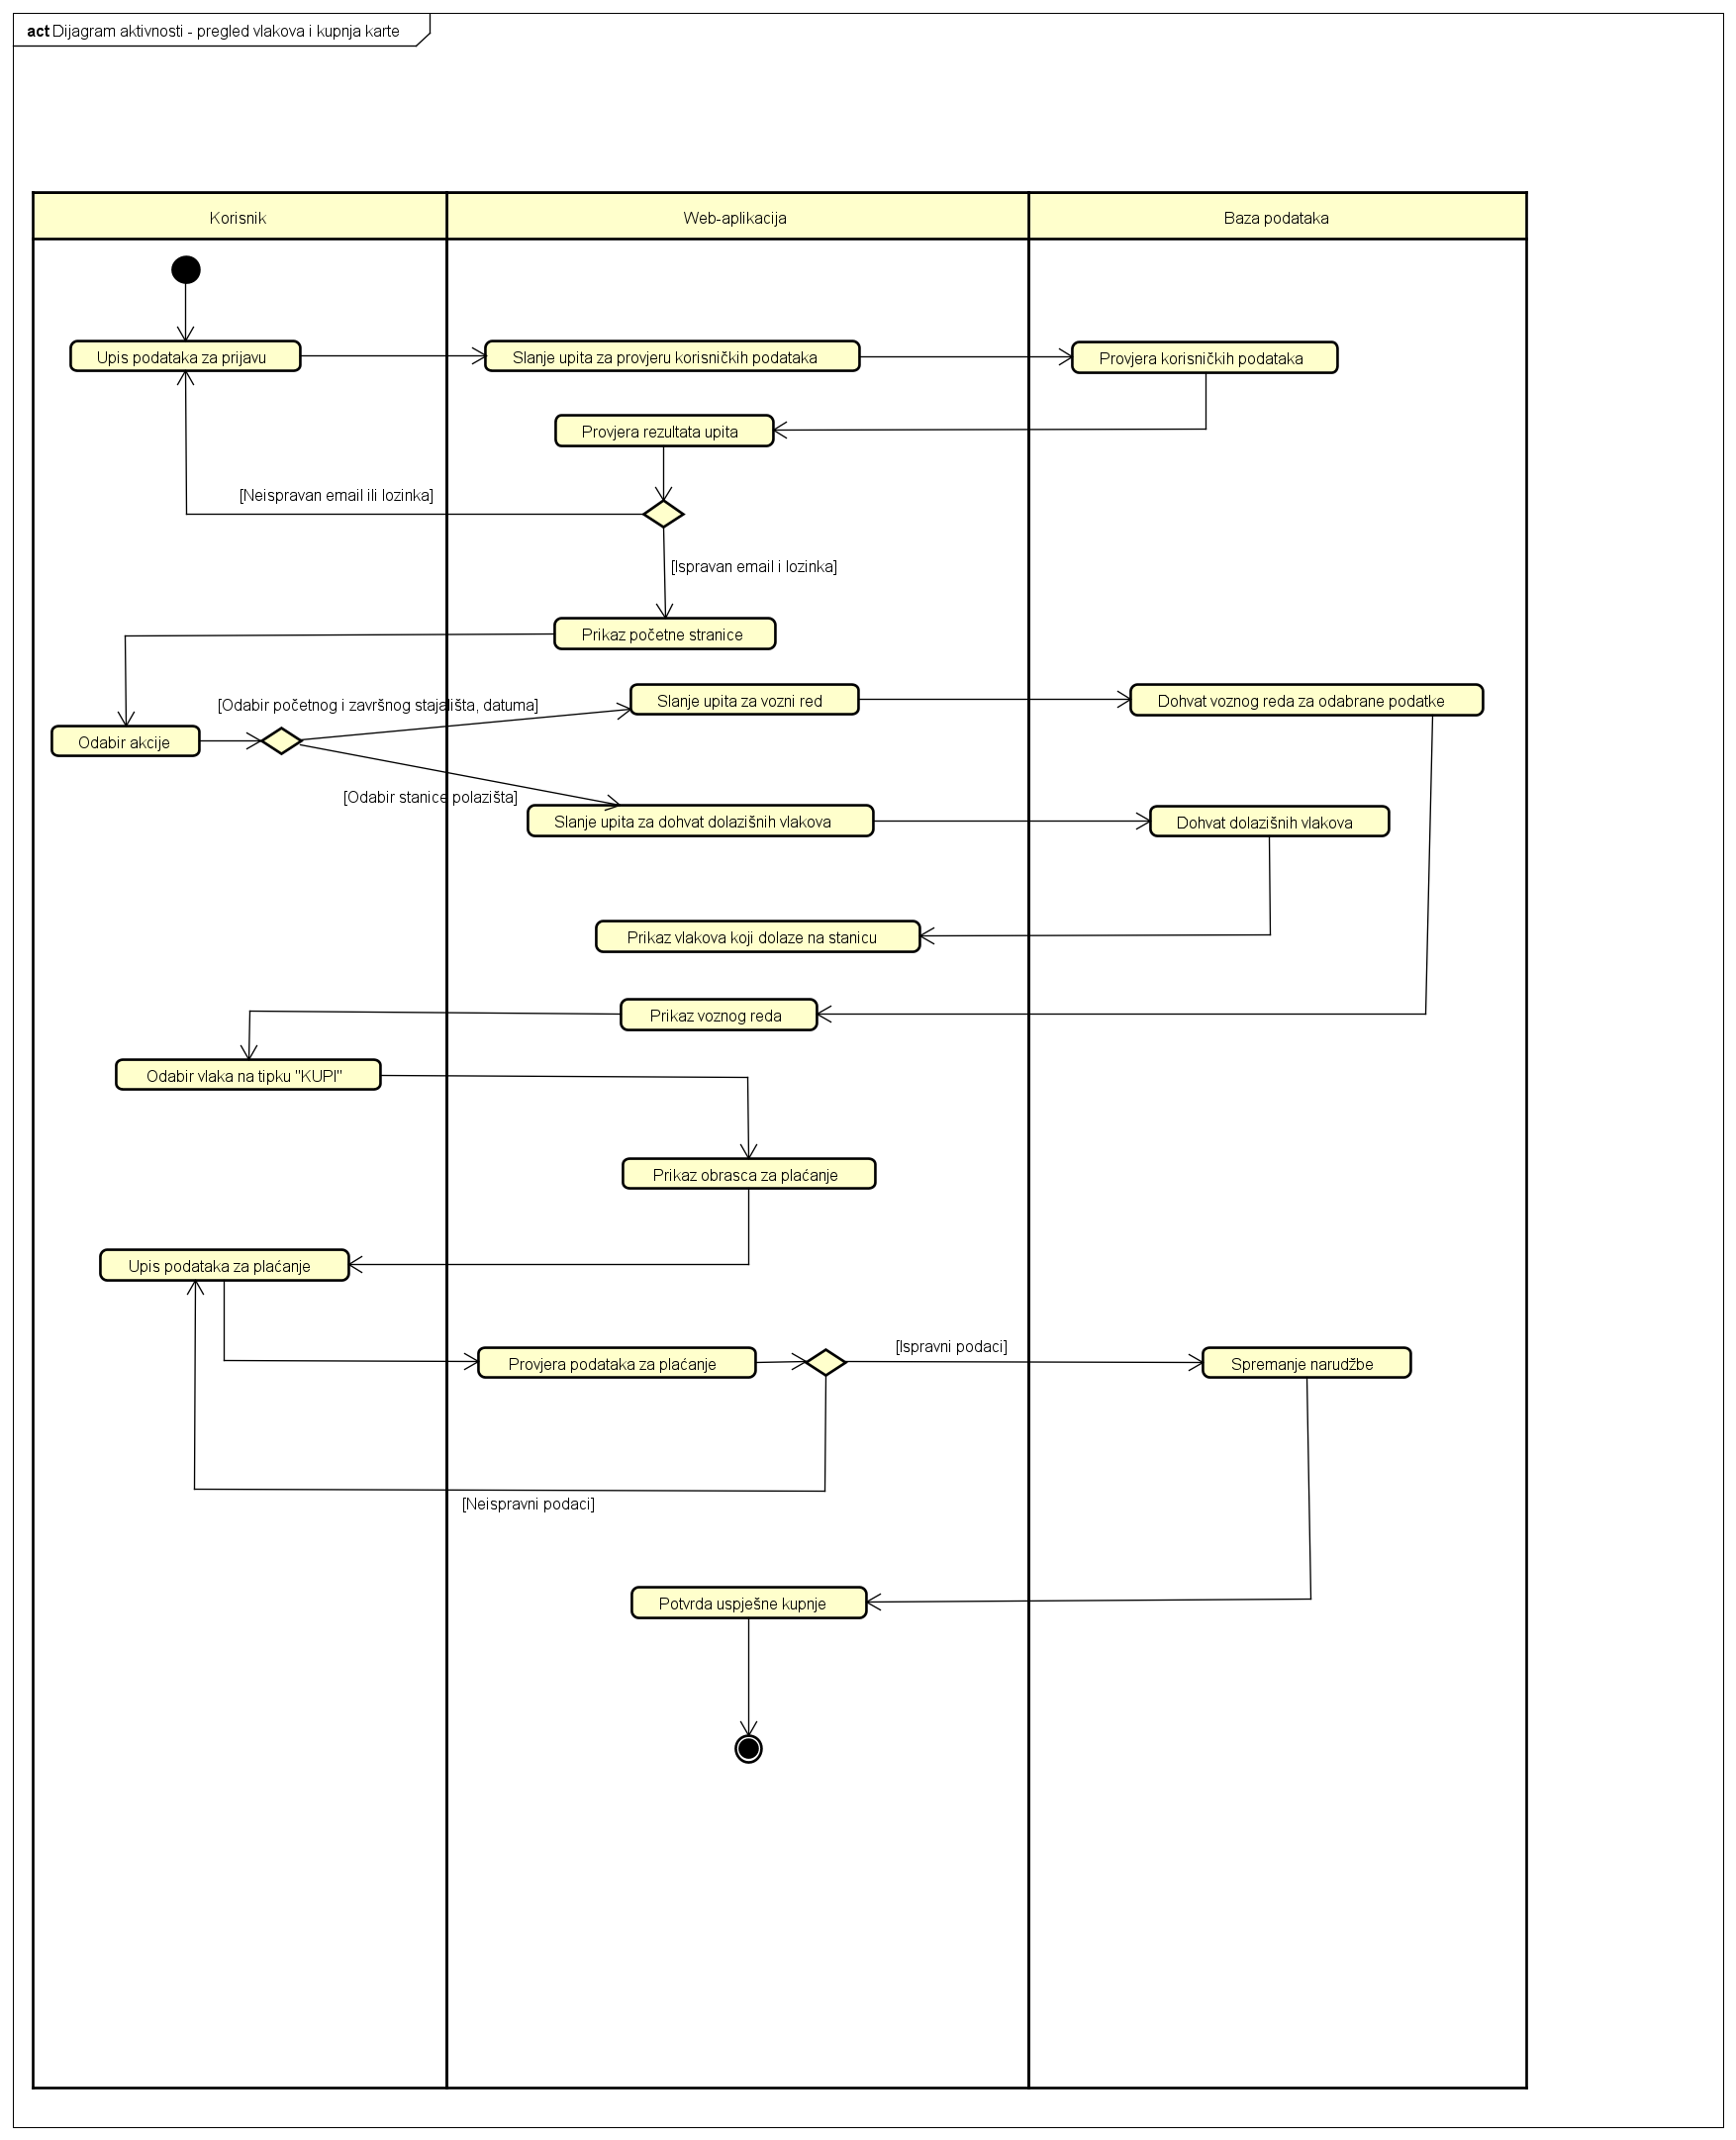
\includegraphics[width=1\linewidth]{"slike/actDiagram1.png"}
					\caption{Dijagram aktivnosti - Pregled vlakova i kupnja karte}
					\label{fig:dij-akt-prvi}
				\end{figure}
			
			% TODO: \usepackage{graphicx} required
				\begin{figure}[H]
					\centering
					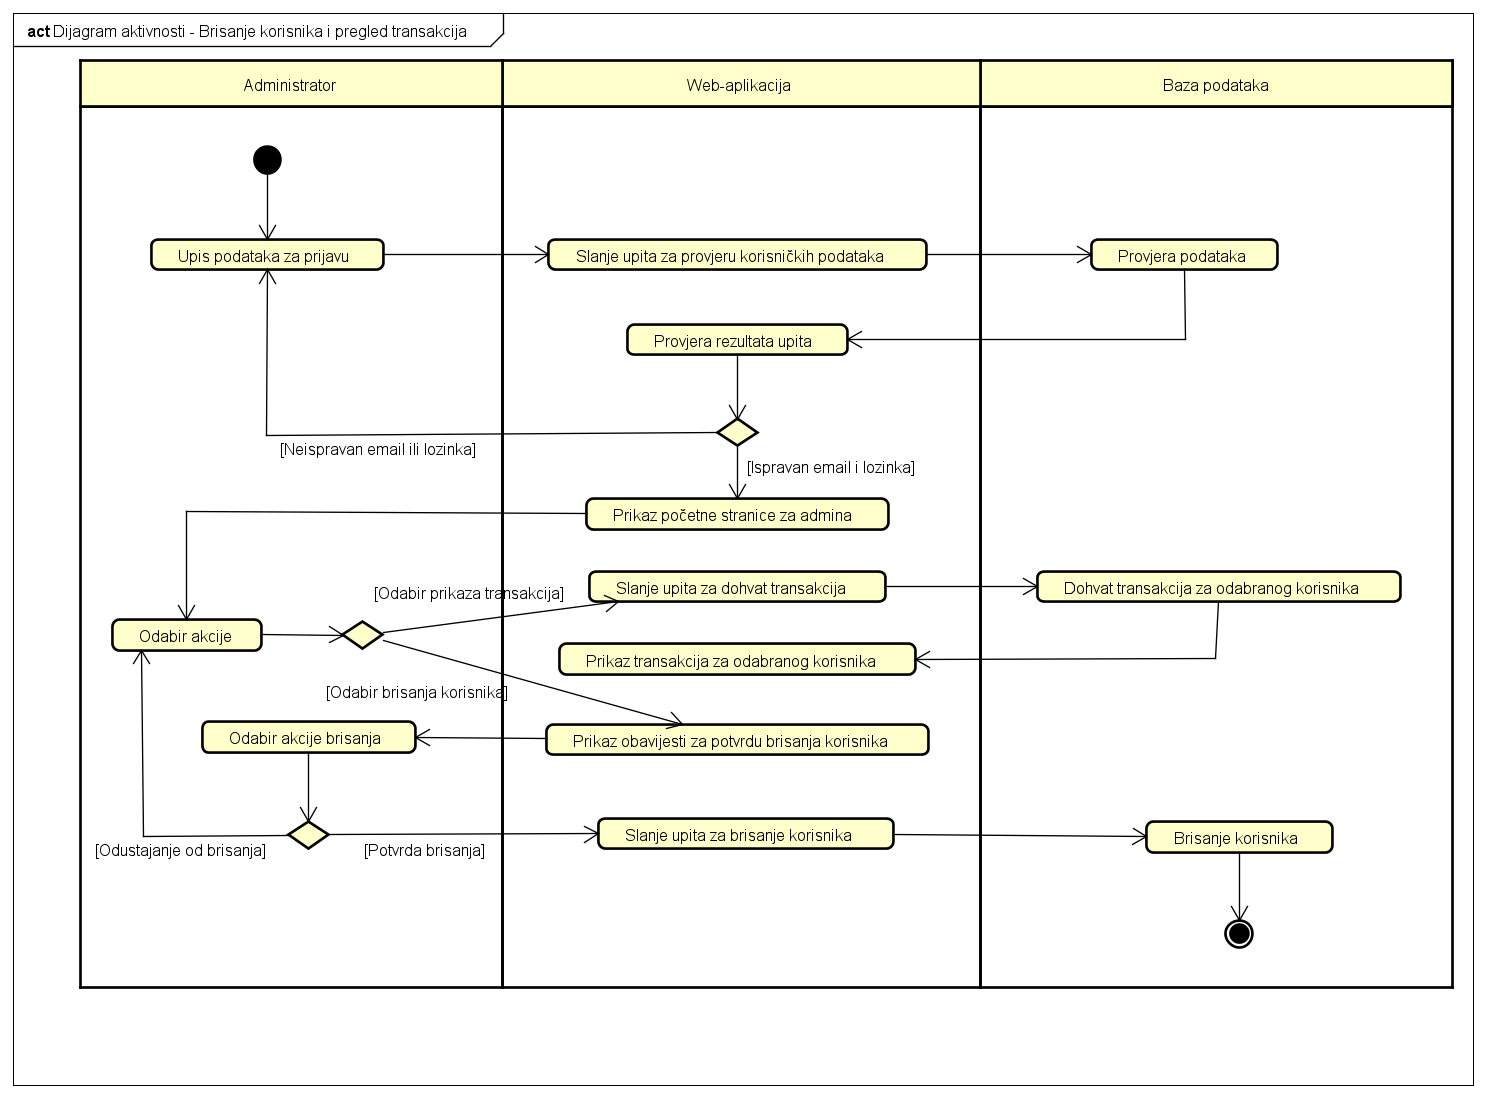
\includegraphics[width=1\linewidth]{"slike/actDiagram2.png"}
					\caption{Dijagram aktivnosti - Brisanje korisnika i pregled transakcija}
					\label{fig:dij-akt-drugi}
				\end{figure}
			
			\eject

\section{Dijagram komponenti}
			{Dijagramom komponenti se vizualizira organizacija i međuovisnost između implementacijskih komponenata te odnos programske potpore prema okolini. Pogodan je za uslužno-orijentiranu arhitekturu i sačinjen je od komponenti, sučelja i poveznica. Sučeljem za dohvat HTML, CSS i JS datoteka dohvaćaju se datoteke sa frontenda aplikacije. Komponentom Router poslužuju se komponente stranice i React biblioteke na upit s URL-a. Dohvatom JSON podataka pristupa se CRUDE REST API komponenti koja komunicira sa backendom aplikacije. Node-Postgres je kolekcija funkcija za komunikaciju Node.js-a i PostgresSQL-a. Pristigli podaci iz baze se šalju MVC arhitekturi u obliku Data transfer object-a.} 
			
			 % TODO: \usepackage{graphicx} required
				\begin{figure}[H]
					\centering
					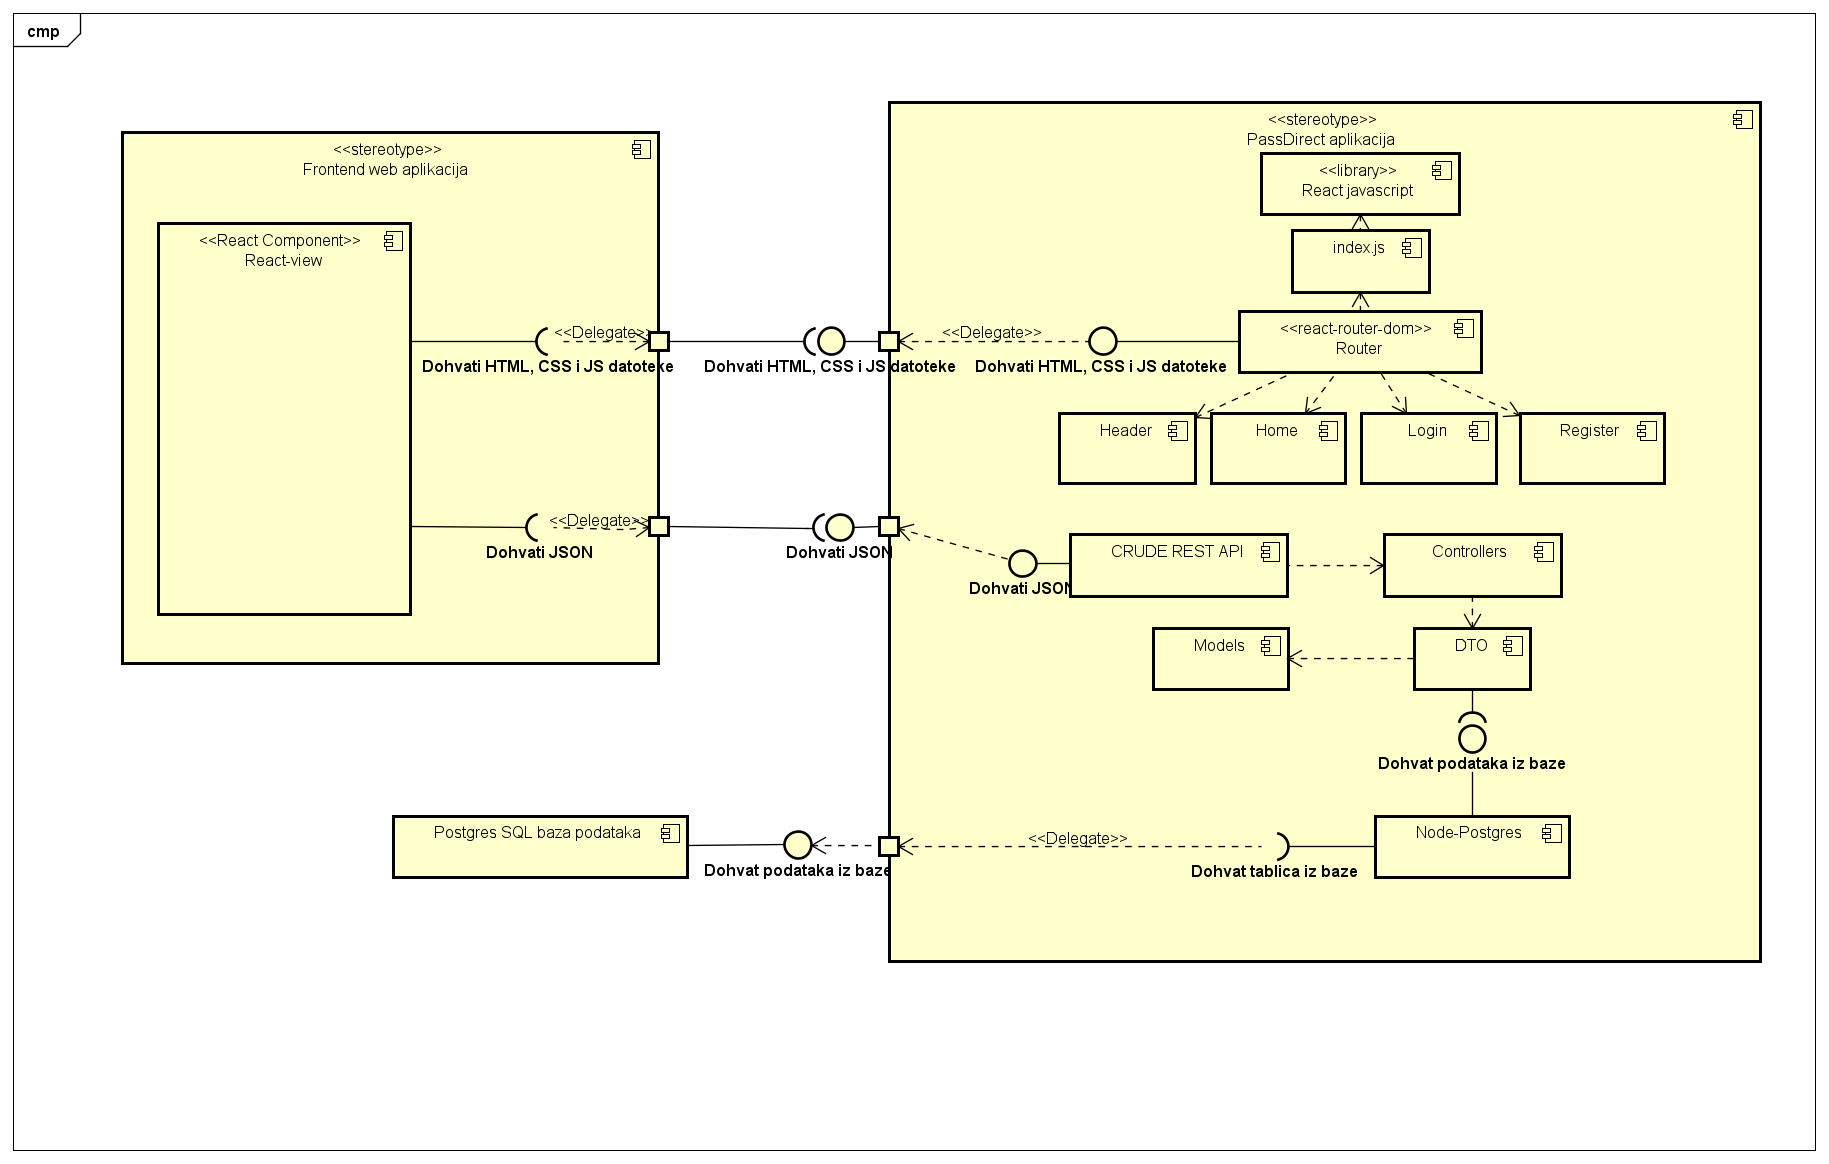
\includegraphics[width=1\linewidth]{"slike/ComponentDiagram.png"}
					\caption{Dijagram komponenti}
					\label{fig:dij-komponenti}
				\end{figure}
			
			
			\eject 
		